% ex: ts=2 sw=2 sts=2 et filetype=tex
% SPDX-License-Identifier: CC-BY-SA-4.0
\begin{frame}
    \frametitle{Contenido}
    \tableofcontents
\end{frame}

\section{Introducción a Python}

\begin{frame}[c]{¿Qué es Python?}
    \begin{columns}
        \column{0.5\textwidth}
        Python es un lenguaje de programación \textit{interpretado} cuya
        filosofía hace hincapié en la \underline{legibilidad de su código}.
        Se trata de un lenguaje de programación \textbf{multiparadigma}, ya
        que soporta parcialmente la \textit{orientación a objetos,
        programación imperativa} y, en menor medida, \textit{programación
        funcional}. \\~\\

        Es un lenguaje interpretado, dinámico y multiplataforma. 
        \column{0.5\textwidth}
        \begin{center}
            
\includegraphics[scale=0.2]{python-logo.png}
        \end{center}
    \end{columns}
\end{frame}

\begin{frame}[c]{Historia}
  \begin{columns}
    \column{0.7\textwidth}
    \begin{itemize}
      \item Creado por Guido Van Rossum
      \item Holanda principios de la decade de los 90's
      \item Sintaxis simple, práctica e intuitiva
      \item De proposito general: NASA, motor de busqueda de Google, Bolsa de
        Valores de Nueva York
      \item Interpretado
      \item Multiparadigma
      \item Tipado dinámico
      \item Python 2.x ya esta \textbf{descontinuado}, solo hay que usar el 3.x
    \end{itemize}
    \column{0.3\textwidth}
        \begin{center}
            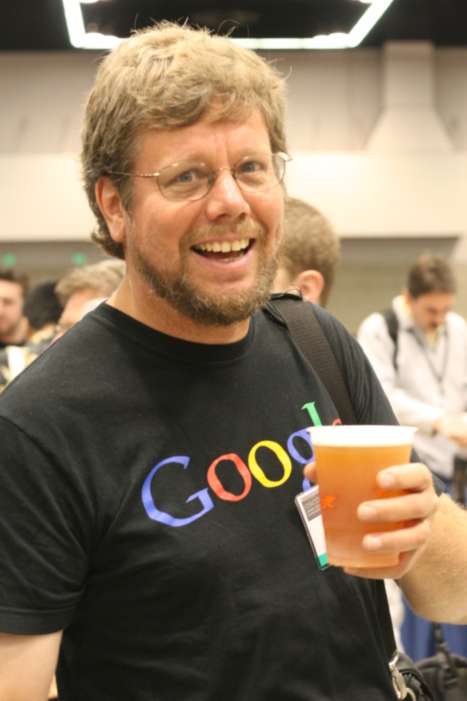
\includegraphics[scale=0.05]{Guido_van_Rossum_OSCON_2006.jpg}
        \end{center}
  \end{columns}
\end{frame}

\begin{frame}[c]{¿Qué puede hacer Python?}
  Python puede:
  \begin{itemize}
    \item ser usado en un servidor para crear aplicaciones web
    \item ser usado junto algún software para crear flojos de trajo.
    \item conectarse a un sistema de base de datos. También puede leer y
          modificar archivos.
    \item ser usado para manejar una gran cantidad de datos y funciones
          matemáticas complejas.
    \item ser usado para el desarrollo de prototipado rápido o para software
          listo para producción.
  \end{itemize}
\end{frame}

\begin{frame}[c]{Ejecución de programas}
  \begin{block}{Código fuente}
    El código generado en Lenguaje Python se almacena en un archivo con
    extensión \textbf{.py}
  \end{block}
\end{frame}

\section{Reglas de codificación}

\begin{frame}[c]{Reglas de codificación}
  \begin{itemize}
    \item Los comentario de una línea inician con "\#"
    \item Los comentarios de varias líneas inician con """ y terminan con """
    \item La sangria cuenta
    \item No poner signos de putuación al final de la instrucción
    \item Es sensible a mayúsculas
    \item Errores de programación:
          \begin{itemize}
            \item Sintaxis
            \item Ejecución
            \item Lógicos
          \end{itemize}
  \end{itemize}
\end{frame}

\begin{frame}[fragile]
  \frametitle{Comentarios en Python}

  Los comentarios pueden ser usados para

  \begin{itemize}
    \item explicar el código de Python.
    \item hacer el código mas legible.
    \item prevenir la ejecución de código de pruebas.
  \end{itemize}

  \begin{lstlisting}[language=Python]
# Este es un comentario
# y otro comentario
print("Hola Mundo")

print("Hola Mundo") # Este es un comentario
# print("Codigo de prueba")

"""
Este es un comentario
escrito en mas
de una sola linea
"""
  \end{lstlisting}
\end{frame}

\section{Variables}

\begin{frame}[fragile]
  \frametitle{Variables en Python}

  Las variables son contenedores para almacenar valores de datos.

  \begin{block}{Creando variables}
    Python no tiene un comando para declarar una variable. \\~\\
    Una variable es \textbf{creada} en el momento que se le asigna un
    valor por primera vez.
  \end{block}

  \begin{lstlisting}[language=Python]
x = 5
y = "Juan"
print(x)
print(y)
  \end{lstlisting}
\end{frame}

\begin{frame}[fragile]
  \frametitle{"Casting" en Python}

  Si se quiere especificar el tipo de dato de una variable, esto se puede hacer
  haciendo "\textbf{casting}"

  \begin{lstlisting}[language=Python]
  x = str(3)   # x guarda '3'
  y = int(3)   # y guarda 3
  z = float(3) # z guarda 3.0
  \end{lstlisting}
\end{frame}

\begin{frame}[fragile]
  \frametitle{Obteniendo el tipo de dato}

  Se puede obtener el tipo de dato con la función \textbf{type()}

  \begin{lstlisting}[language=Python]
  x = str(3)   # x guarda '3'
  y = int(3)   # y guarda 3
  z = float(3) # z guarda 3.0

  print( type(x) )
  print( type(y) )
  print( type(z) )
  \end{lstlisting}
\end{frame}

\begin{frame}[fragile,b]
  \frametitle{Nombre de variables}

  Las variables pueden tener un nombre corto (como \textit{x} y \textit{y})
  o tener un nombre más \textbf{descriptivo} (\textit{edad}, \textit{nombre} 
  \textit{volumen\_total}). Las reglas para las variables en Python son:

  \begin{itemize}
    \item El nombre de la variable tiene que \textbf{comenzar} con una
      \textbf{letra} o un \textbf{guión bajo} (\_).
    \item El nombre de una variable \textbf{no} puede iniciar con
      \textit{número.}
    \item El nombre de una variable solo puede contener caracteres
      alfa-numéricos y guiones bajo (\textit{A-Z, a-z, 0-9 y "\_"})
    \item Los nombre de las variables son sensibles a mayúsculas y minúsculas
      (edad, Edad y EDAD son tres variables deferentes)
  \end{itemize}

  \begin{lstlisting}[language=Python]
    myvar = "Juan"
    my_var = "Juan"
    _my_var = "Juan"
    myVar = "Juan"
    MYVAR = "Juan"
    myvar2 = "Juan"
  \end{lstlisting}
\end{frame}

\begin{frame}[c]{Variables con múltiples palabras}
  Un nombre de una variable con múltiples palabras puede ser difícil de leer.
  Hay varias técnicas que se pueden usar para que sean mas legibles.
  \begin{block}{Camel case}
    Cada palabra, excepto la primera, comienza con una mayúscula:
    \textbf{elNombreDeMiVariable}
  \end{block}
  \begin{block}{Pascal case}
    Cada palabra comienza con una mayúscula:
    \textbf{ElNombreDeMiVariable}
  \end{block}
  \begin{block}{Snake case}
    Cada palabra esta separada por un guión bajo:
    \textbf{el\_nombre\_de\_mi\_variable}
  \end{block}
\end{frame}

\begin{frame}[fragile]
  \frametitle{Asignando múltiples variables}

  Python permite asignar valores a múltiples variables en una sola linea:

  \begin{lstlisting}[language=Python]
  color, sabor, olor = "azul", "dulce", "rosas"
  print(color)
  print(sabor)
  print(olor)
  \end{lstlisting}

  \begin{block}{Nota}
    Hay que asegurar que el número de variables sea igual al número de valores
    asignados, ya que de lo contrario se podría generar un error.
  \end{block}
\end{frame}

\begin{frame}[fragile]
  \frametitle{Un valor para múltiples variables}

  También se puede asignar el mismo valor a múltiples variables en una sola
  línea.

  \begin{lstlisting}[language=Python]
  x = y = z = "Manzana"
  print(x)
  print(y)
  print(z)
  \end{lstlisting}

\end{frame}

\begin{frame}[fragile]
  \frametitle{Vaciar una Colección}

  Si se tiene una colección de valores en una \textit{lista}, \textit{tupla},
  etc. Python permite extraer los valores en variables separadas. A esto
  se le llama en ingles \textbf{unpacking}

  \begin{lstlisting}[language=Python]
  frutas = ["manzana", "platano", "melon"]
  a, b, c = frutas
  print(a)
  print(b)
  print(c)
  \end{lstlisting}

\end{frame}
